% First-quadrant representations of 65; coordinates are exact integers.
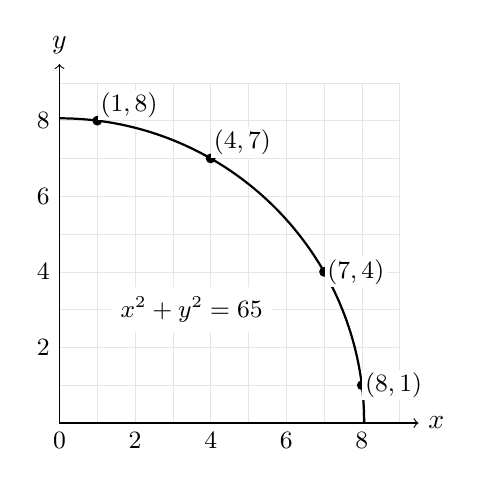
\begin{tikzpicture}[scale=.48]
\draw[step=1,gray!20,very thin] (0,0) grid (9,9);
\draw[->] (0,0)--(9.5,0) node[right] {$x$};
\draw[->] (0,0)--(0,9.5) node[above] {$y$};
\draw[thick] (8.062258,0) arc[start angle=0,end angle=90,radius=8.062258];
\foreach \x in {0,2,4,6,8} {\node[below,font=\small] at (\x,0) {\x};}
\foreach \y in {2,4,6,8} {\node[left,font=\small] at (0,\y) {\y};}
\foreach \x/\y in {1/8,4/7,7/4,8/1} {\fill (\x,\y) circle[radius=.13];}
\node[above right,font=\small,fill=white,inner sep=1pt] at (1,8) {$(1,8)$};
\node[above right,font=\small,fill=white,inner sep=1pt] at (4,7) {$(4,7)$};
\node[right,font=\small,fill=white,inner sep=1pt] at (7,4) {$(7,4)$};
\node[right,font=\small,fill=white,inner sep=1pt] at (8,1) {$(8,1)$};
\node[font=\small,fill=white] at (3.5,3) {$x^2+y^2=65$};
\end{tikzpicture}
